%%%%%%%%%%%%%%%%%%%%%%%%%%%%%%%%%%%%%%%%%
% Cleese Assignment (For Students)
% LaTeX Template
% Version 2.0 (27/5/2018)
%
% This template originates from:
% http://www.LaTeXTemplates.com
%
% Author:
% Vel (vel@LaTeXTemplates.com)
%
% License:
% CC BY-NC-SA 3.0 (http://creativecommons.org/licenses/by-nc-sa/3.0/)
% 
%%%%%%%%%%%%%%%%%%%%%%%%%%%%%%%%%%%%%%%%%

%----------------------------------------------------------------------------------------
%	PACKAGES AND OTHER DOCUMENT CONFIGURATIONS
%----------------------------------------------------------------------------------------

\documentclass[11pt]{article}

%%%%%%%%%%%%%%%%%%%%%%%%%%%%%%%%%%%%%%%%%
% Cleese Assignment
% Structure Specification File
% Version 1.0 (27/5/2018)
%
% This template originates from:
% http://www.LaTeXTemplates.com
%
% Author:
% Vel (vel@LaTeXTemplates.com)
%
% License:
% CC BY-NC-SA 3.0 (http://creativecommons.org/licenses/by-nc-sa/3.0/)
% 
%%%%%%%%%%%%%%%%%%%%%%%%%%%%%%%%%%%%%%%%%

%----------------------------------------------------------------------------------------
%	PACKAGES AND OTHER DOCUMENT CONFIGURATIONS
%----------------------------------------------------------------------------------------

\usepackage{lastpage} % Required to determine the last page number for the footer

\usepackage{graphicx} % Required to insert images

\setlength\parindent{0pt} % Removes all indentation from paragraphs

\usepackage[most]{tcolorbox} % Required for boxes that split across pages

\usepackage{booktabs} % Required for better horizontal rules in tables

\usepackage{listings} % Required for insertion of code

\usepackage{etoolbox} % Required for if statements

% Manujinda
\usepackage{float}
\usepackage{subcaption}
\usepackage{amsmath}
\usepackage{mathtools}
\usepackage{xfrac}
\usepackage{multirow}
\usepackage{xcolor}
%\usepackage{hyperref}
\usepackage[colorlinks=true,linkcolor=blue,urlcolor=cyan,bookmarks=true,bookmarksopen=true]{hyperref}
%\usepackage[open,openlevel=1]{bookmark}

%\usepackage[latin1]{inputenc}
\usepackage{tikz}
\usetikzlibrary{trees}
\usetikzlibrary{bayesnet}
\usepackage{verbatim}
\usepackage{physics} % To have differentiation stuff dy/dx
\usepackage{cancel} % To cross off terms with an arrow and a simplified term
\usepackage{amssymb} % To get the null set symbol
% To have equation numbers in the align* environment
\newcommand\numberthis{\addtocounter{equation}{1}\tag{\theequation}}

%----------------------------------------------------------------------------------------
%	MARGINS
%----------------------------------------------------------------------------------------

\usepackage{geometry} % Required for adjusting page dimensions and margins

\geometry{
	paper=a4paper, % Change to letterpaper for US letter
	top=3cm, % Top margin
	bottom=3cm, % Bottom margin
	left=2.5cm, % Left margin
	right=2.5cm, % Right margin
	headheight=14pt, % Header height
	footskip=1.4cm, % Space from the bottom margin to the baseline of the footer
	headsep=1.2cm, % Space from the top margin to the baseline of the header
	%showframe, % Uncomment to show how the type block is set on the page
}

%----------------------------------------------------------------------------------------
%	FONT
%----------------------------------------------------------------------------------------

\usepackage[utf8]{inputenc} % Required for inputting international characters
\usepackage[T1]{fontenc} % Output font encoding for international characters

\usepackage[sfdefault,light]{roboto} % Use the Roboto font

%----------------------------------------------------------------------------------------
%	HEADERS AND FOOTERS
%----------------------------------------------------------------------------------------

\usepackage{fancyhdr} % Required for customising headers and footers

\pagestyle{fancy} % Enable custom headers and footers

\lhead{\small\assignmentClass\ifdef{\assignmentClassInstructor}{\ (\assignmentClassInstructor):}{}\ \assignmentTitle} % Left header; output the instructor in brackets if one was set
\chead{} % Centre header
\rhead{\small\ifdef{\assignmentAuthorName}{\assignmentAuthorName}{\ifdef{\assignmentDueDate}{Due\ \assignmentDueDate}{}}} % Right header; output the author name if one was set, otherwise the due date if that was set

\lfoot{} % Left footer
\cfoot{\small Page\ \thepage\ of\ \pageref{LastPage}} % Centre footer
\rfoot{} % Right footer

\renewcommand\headrulewidth{0.5pt} % Thickness of the header rule

%----------------------------------------------------------------------------------------
%	MODIFY SECTION STYLES
%----------------------------------------------------------------------------------------

\usepackage{titlesec} % Required for modifying sections

%------------------------------------------------
% Section

\titleformat
{\section} % Section type being modified
[block] % Shape type, can be: hang, block, display, runin, leftmargin, rightmargin, drop, wrap, frame
{\Large\bfseries} % Format of the whole section
{\assignmentQuestionName~\thesection} % Format of the section label
{6pt} % Space between the title and label
{} % Code before the label

\titlespacing{\section}{0pt}{0.5\baselineskip}{0.5\baselineskip} % Spacing around section titles, the order is: left, before and after

%------------------------------------------------
% Subsection

\titleformat
{\subsection} % Section type being modified
[block] % Shape type, can be: hang, block, display, runin, leftmargin, rightmargin, drop, wrap, frame
{\itshape} % Format of the whole section
{(\alph{subsection})} % Format of the section label
{4pt} % Space between the title and label
{} % Code before the label

\titlespacing{\subsection}{0pt}{0.5\baselineskip}{0.5\baselineskip} % Spacing around section titles, the order is: left, before and after

\renewcommand\thesubsection{(\alph{subsection})}

%----------------------------------------------------------------------------------------
%	CUSTOM QUESTION COMMANDS/ENVIRONMENTS
%----------------------------------------------------------------------------------------

% Environment to be used for each question in the assignment
\newenvironment{question}{
	\vspace{0.5\baselineskip} % Whitespace before the question
	\section{} % Blank section title (e.g. just Question 2)
	\lfoot{\small\itshape\assignmentQuestionName~\thesection~continued on next page\ldots} % Set the left footer to state the question continues on the next page, this is reset to nothing if it doesn't (below)
}{
	\lfoot{} % Reset the left footer to nothing if the current question does not continue on the next page
}

%------------------------------------------------

% Environment for subquestions, takes 1 argument - the name of the section
\newenvironment{subquestion}[1]{
	\subsection{#1}
}{
}

%------------------------------------------------

% Command to print a question sentence
\newcommand{\questiontext}[1]{
	\textbf{#1}
	\vspace{0.5\baselineskip} % Whitespace afterwards
}

%------------------------------------------------

% Command to print a box that breaks across pages with the question answer
\newcommand{\answer}[1]{
	\begin{tcolorbox}[breakable, enhanced]
		#1
	\end{tcolorbox}
}

%------------------------------------------------

% Command to print a box that breaks across pages with the space for a student to answer
\newcommand{\answerbox}[1]{
	\begin{tcolorbox}[breakable, enhanced]
		\vphantom{L}\vspace{\numexpr #1-1\relax\baselineskip} % \vphantom{L} to provide a typesetting strut with a height for the line, \numexpr to subtract user input by 1 to make it 0-based as this command is
	\end{tcolorbox}
}

%------------------------------------------------

% Command to print an assignment section title to split an assignment into major parts
\newcommand{\assignmentSection}[1]{
	{
		\centering % Centre the section title
		\vspace{2\baselineskip} % Whitespace before the entire section title
		
		\rule{0.8\textwidth}{0.5pt} % Horizontal rule
		
		\vspace{0.75\baselineskip} % Whitespace before the section title
		{\LARGE \MakeUppercase{#1}} % Section title, forced to be uppercase
		
		\rule{0.8\textwidth}{0.5pt} % Horizontal rule
		
		\vspace{\baselineskip} % Whitespace after the entire section title
	}
}

%----------------------------------------------------------------------------------------
%	TITLE PAGE
%----------------------------------------------------------------------------------------

\author{\textbf{\assignmentAuthorName}} % Set the default title page author field
\date{} % Don't use the default title page date field

\title{
	\thispagestyle{empty} % Suppress headers and footers
	\vspace{0.2\textheight} % Whitespace before the title
	\textbf{\assignmentClass:\ \assignmentTitle}\\[-4pt]
	\ifdef{\assignmentDueDate}{{\small Due\ on\ \assignmentDueDate}\\}{} % If a due date is supplied, output it
	\ifdef{\assignmentClassInstructor}{{\large \textit{\assignmentClassInstructor}}}{} % If an instructor is supplied, output it
	\vspace{0.32\textheight} % Whitespace before the author name
}
 % Include the file specifying the document structure and custom commands

%----------------------------------------------------------------------------------------
%	ASSIGNMENT INFORMATION
%----------------------------------------------------------------------------------------

% Required
\newcommand{\assignmentQuestionName}{Question} % The word to be used as a prefix to question numbers; example alternatives: Problem, Exercise
\newcommand{\assignmentClass}{CSC 535} % Course/class
\newcommand{\assignmentTitle}{Assignment \#6} % Assignment title or name
\newcommand{\assignmentAuthorName}{Ariyan, Manujinda, Marina} % Student name

% Optional (comment lines to remove)
\newcommand{\assignmentClassInstructor}{Kobus Barnard} % Intructor name/time/description
\newcommand{\assignmentDueDate}{Wednesday,\ October\ 31,\ 2018} % Due date

%----------------------------------------------------------------------------------------

\begin{document}

%----------------------------------------------------------------------------------------
%	TITLE PAGE
%----------------------------------------------------------------------------------------

\maketitle % Print the title page

\thispagestyle{empty} % Suppress headers and footers on the title page

\newpage

\paragraph{}
\textbf{}

%----------------------------------------------------------------------------------------
%	QUESTION 1
%----------------------------------------------------------------------------------------

\begin{question}

	\questiontext{Probability table}

	\begin{subquestion}{Produce the $9 \times 9$ table $p(measured\_angle \mid angle)$}
		\answer{
			\begin{table}[H]
				\centering
				\caption{$p(measured\_angle \mid angle)$}
				\label{tbl:ma-given-a}
				\begin{tabular}{c c r r r r r r r r r}
					\toprule
					&  	& \multicolumn{9}{c}{\textbf{Measured Angle}} \\
					&  	& \multicolumn{1}{c}{$\mathbf{1}$} & \multicolumn{1}{c}{$\mathbf{2}$}  & \multicolumn{1}{c}{$\mathbf{3}$} & \multicolumn{1}{c}{$\mathbf{4}$} & \multicolumn{1}{c}{$\mathbf{5}$} & \multicolumn{1}{c}{$\mathbf{6}$} & \multicolumn{1}{c}{$\mathbf{7}$} & \multicolumn{1}{c}{$\mathbf{8}$} & \multicolumn{1}{c}{$\mathbf{9}$} \\
					\midrule
					%\multirow{9}*{\textbf{Model (True) angle}} 	
					\parbox[t]{2mm}{\multirow{9}{*}{\rotatebox[origin=c]{90}{\textbf{Model (True) angle}}}}
						& $\mathbf{1}$ & $0.7$ & $0.2$ & $0.1$ & $0$ & $0$ & $0$ & $0$ & $0$ & $0$ \\
						& $\mathbf{2}$ & $0.3$ & $0.4$ & $0.2$ & $0.1$ & $0$ & $0$ & $0$ & $0$ & $0$ \\
						& $\mathbf{3}$ & $0.1$ & $0.2$ & $0.4$ & $0.2$ & $0.1$ & $0$ & $0$ & $0$ & $0$ \\
						& $\mathbf{4}$ & $0$ & $0.1$ & $0.2$ & $0.4$ & $0.2$ & $0.1$ & $0$ & $0$ & $0$ \\
						& $\mathbf{5}$ & $0$ & $0$ & $0.1$ & $0.2$ & $0.4$ & $0.2$ & $0.1$ & $0$ & $0$ \\
						& $\mathbf{6}$ & $0$ & $0$ & $0$ & $0.1$ & $0.2$ & $0.4$ & $0.2$ & $0.1$ & $0$ \\
						& $\mathbf{7}$ & $0$ & $0$ & $0$ & $0$ & $0.1$ & $0.2$ & $0.4$ & $0.2$ & $0.1$ \\
						& $\mathbf{8}$ & $0$ & $0$ & $0$ & $0$ & $0$ & $0.1$ & $0.2$ & $0.4$ & $0.3$ \\
						& $\mathbf{9}$ & $0$ & $0$ & $0$ & $0$ & $0$ & $0$ & $0.1$ & $0.2$ & $0.7$ \\
					\bottomrule
				\end{tabular}
			\end{table}
		}
	\end{subquestion}

	%\pagebreak
	\begin{subquestion}{Variance of the measurements}

		\answer{
		}
	\end{subquestion}

\end{question}


%----------------------------------------------------------------------------------------
%	QUESTION 2
%----------------------------------------------------------------------------------------
\pagebreak
\begin{question}

	\questiontext{Graphical Model}

%	\begin{subquestion}{The Bayes Net}
		\answer{
			\begin{figure}[H] 
				\begin{center}
					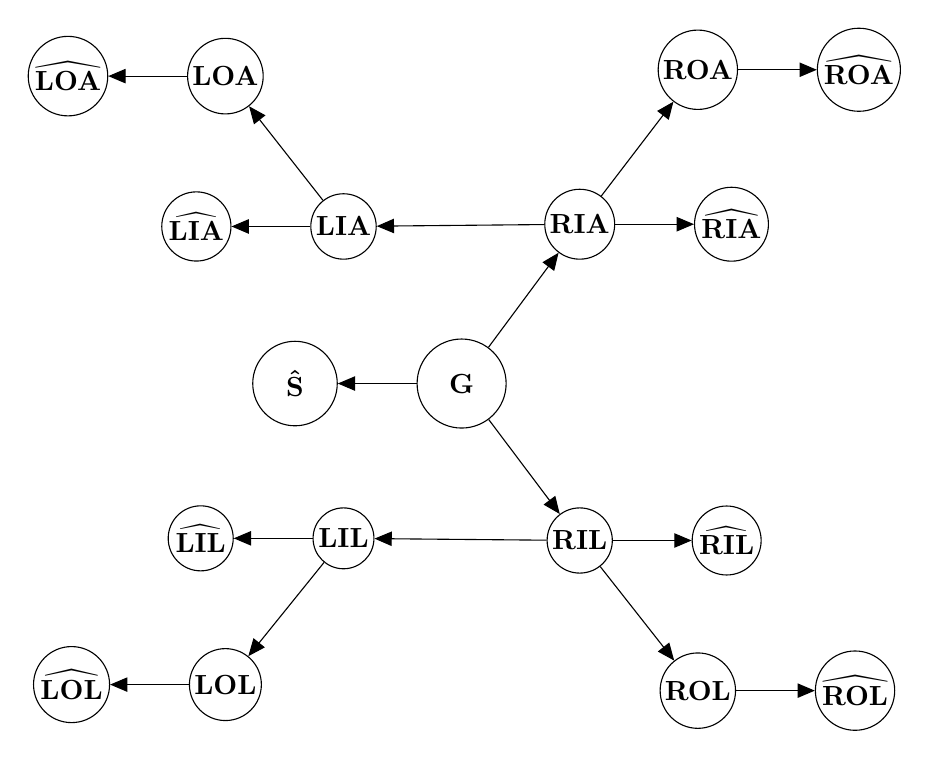
\begin{tikzpicture}
					\node[latent]                            (G) {$\mathbf{\quad G \quad }$};
					\node[latent, above=of G, xshift=-1.5cm] (LIA) {$\mathbf{LIA}$};
					\node[latent, above=of G, xshift= 1.5cm] (RIA) {$\mathbf{RIA}$};
					\node[latent, above=of LIA, xshift=-1.5cm] (LOA) {$\mathbf{LOA}$};
					\node[latent, above=of RIA, xshift= 1.5cm] (ROA) {$\mathbf{ROA}$};
					\node[latent, below=of G, xshift=-1.5cm] (LIL) {$\mathbf{LIL}$};
					\node[latent, below=of G, xshift= 1.5cm] (RIL) {$\mathbf{RIL}$};
					\node[latent, below=of LIL, xshift=-1.5cm] (LOL) {$\mathbf{LOL}$};
					\node[latent, below=of RIL, xshift= 1.5cm] (ROL) {$\mathbf{ROL}$};

					% Observations
					\node[latent, left=of G] (hS) {$\mathbf{\quad \hat S\quad}$};
					\node[latent, left=of LIA] (hLIA) {$\mathbf{\widehat {LIA}}$};
					\node[latent, left=of LOA] (hLOA) {$\mathbf{\widehat {LOA}}$};
					\node[latent, left=of LIL] (hLIL) {$\mathbf{\widehat {LIL}}$};
					\node[latent, left=of LOL] (hLOL) {$\mathbf{\widehat {LOL}}$};
					\node[latent, right=of RIA] (hRIA) {$\mathbf{\widehat {RIA}}$};
					\node[latent, right=of ROA] (hROA) {$\mathbf{\widehat {ROA}}$};
					\node[latent, right=of RIL] (hRIL) {$\mathbf{\widehat {RIL}}$};
					\node[latent, right=of ROL] (hROL) {$\mathbf{\widehat {ROL}}$};

					% Connect the nodes
					\edge {G} {RIA, RIL, hS};
					\edge {RIA} {ROA, LIA, hRIA};
					\edge {LIA} {LOA, hLIA};
					\edge {RIL} {ROL, LIL, hRIL};
					\edge {LIL} {LOL, hLIL};
					\edge {ROA} {hROA}
					\edge {LOA} {hLOA}
					\edge {ROL} {hROL}
					\edge {LOL} {hLOL}
					\end{tikzpicture}
				\end{center}
		\end{figure}
		}		  
%	\end{subquestion}
\end{question}


%----------------------------------------------------------------------------------------
%	QUESTION 3
%----------------------------------------------------------------------------------------
%\pagebreak
\begin{question}
	\questiontext{Formula for the joint distribution}

	%\begin{subquestion}{Formula for the joint distribution}
		\answer{
			\begin{align*}
				p(G, \hat S, RIA, RIL, ROA, ROL, \\ LIA, LIL, LOA, LOL, \\ \widehat {RIA}, \widehat {RIL}, \widehat {ROA}, \widehat {ROL}, \\ \widehat {LIA}, \widehat {LIL}, \widehat {LOA}, \widehat {LOL}) =& p(G)p(\hat S \mid G)p(RIA \mid G)p(RIL \mid G) \\
					 & p(LIA \mid RIA)p(ROA \mid RIA)p(LOA \mid LIA) \\
					 & p(LIL \mid RIL)p(ROL \mid RIL)p(LOL \mid LIL) \\
					 & p(\widehat {RIA} \mid RIA)p(\widehat {ROA} \mid ROA)p(\widehat {RIL} \mid RIL)p(\widehat {ROL} \mid ROL) \\
					 & p(\widehat {LIA} \mid LIA)p(\widehat {LOA} \mid LOA)p(\widehat {LIL} \mid LIL)p(\widehat {LOL} \mid LOL)
			\end{align*}
		}
	%\end{subquestion}
\end{question}


\pagebreak
%----------------------------------------------------------------------------------------
%	QUESTION 4
%----------------------------------------------------------------------------------------

\newcommand{\sample}[1]{%
	\begin{subfigure}[H]{0.45\textwidth}
		\includegraphics[width=\textwidth]{Sample-#1-Actual.png}
	\end{subfigure}
	~ %add desired spacing between images, e. g. ~, \quad, \qquad, \hfill etc. 
	%(or a blank line to force the subfigure onto a new line)
	\begin{subfigure}[H]{0.45\textwidth}
		\includegraphics[width=\textwidth]{Sample-#1-Observed.png}
	\end{subfigure}
	\\
}

\begin{question}

	\questiontext{Generated samples}

	%\begin{subquestion}{Generated samples}
		\begin{figure}[H]
			\center
			\sample{1}
			\sample{2}
			\sample{3}
			\caption{Generated samples 1 - 3 for idealized individuals and observed appearance.}
			\label{fig:samples}
		\end{figure}

		\begin{figure}[H]
			\center
			\sample{4}
			\sample{5}
			\sample{6}
			\sample{7}
			\caption{Generated samples 4 - 7 for idealized individuals and observed appearance.}
			\label{fig:samples}
		\end{figure}

		\begin{figure}[H]
			\center
			\sample{8}
			\sample{9}
			\sample{10}
			\caption{Generated samples 8 - 10 for idealized individuals and observed appearance.}
			\label{fig:samples}
		\end{figure}
	%\end{subquestion}
\end{question}


%----------------------------------------------------------------------------------------
%	QUESTION 5
%----------------------------------------------------------------------------------------
%\pagebreak
\begin{question}

	\questiontext{Deciding gender of MQLs from images}

	\begin{subquestion}{From image of idealized individuals}
			\answer{
			}		  
	\end{subquestion}

	\begin{subquestion}{From image of observed appearance}
		\answer{
		}		  
	\end{subquestion}
\end{question}


%----------------------------------------------------------------------------------------
%	QUESTION 6
%----------------------------------------------------------------------------------------
%\pagebreak
\begin{question}

	\questiontext{Generating synthetic data to experiment with inference}

	\begin{subquestion}{xxx}
			\answer{
			}		  
	\end{subquestion}

\end{question}

%----------------------------------------------------------------------------------------

\end{document}
